\documentclass[a4paper,10pt]{article}
\usepackage{hyperref}
\usepackage{geometry}
\usepackage{graphicx}
\usepackage[sort]{natbib}
\geometry{a4paper,left=1.5cm,right=1.5cm,top=3cm,bottom=4cm}

\title{Notes on DSO}
\author{Xiang Gao}
\date{\today}

\begin{document}
	\maketitle
	
	\begin{quotation}
		\centering
		Listen, my friend: the ages that are past
		
		Are now a book with seven seals protected:
		
		What you the Spirit of the Ages call
		
		Is nothing but the spirit of you all,
		
		Wherein the Ages are reflected.
		
		--Faust, Johann Wolfgang Von Goethe
	\end{quotation}
	
	\section{Introduction on DSO}
	\subsection{What is DSO}
	DSO (Direct Sparse Odometry) is a visual odometry system published in 2016 by Dr. Jakob Engel from the Computer Vision Laboratory at the Technical University of Munich (TUM) \cite{engel2017direct}. For the laboratory home page, see \url{https://vision.in.tum.de/research/vslam/dso}. The code link is here: \url{https://github.com/JakobEngel/dso}. For now there are many different versions of DSO like stereo DSO, IMU-integrated DSO, DSO with loop closing, DSO with auto photometric calibration, DSO with rolling shutter camera, etc. Some of them are from our CV group and the others are from public community. Unfortunately, our group only releases the basic DSO version, and if you are interested on stereo DSO or IMU-DSO, please look for other open-source versions in the website, like \url{https://github.com/HorizonAD/stereo_dso}. 

	DSO is already well-explained in the paper of \cite{engel2017direct}, however the code of DSO is not very clearly-written compared to other open-source systems like ORB-SLAM2 and SVO (thanks to Jakob), which makes it very difficult for researchers (and me) to conduct follow-up research based on it. This note is to explain some of the basic knowledges about DSO's code, like how it is organized, what is the working pipeline of DSO, etc. 
	
	In order to understand this note you should at least have the basic knowledge of visual SLAM, like 3D rigid-body motion and bundle adjustment. You'd better read the DSO's paper at first before reading this material.
	
	\subsection{Direct method}
	DSO is a keyframe visual odometry based on direct method. It is \textbf{not} a complete SLAM system and does not include loop closing detection or map reusing, which means it \emph{won't} reuse the previously built map. DSO keeps a small window of active keyframes (sometimes called \textbf{Sliding Window Filter} (SWF) algorithm), Once a keyframe is out of the active window, you cannot use its information anymore (which is called as \textbf{Marginalization} and we will explain it later). Therefore, it inevitably has accumulative errors (on rotation, translation, and scale), which are small but cannot be eliminated. 
	
	DSO is one of the few visual odometry systems using fully direct method. In contrast, SVO \cite{forster2014svo} is a semi-direct method which use direct tracking as the front-end but still minimizes the geometry error in back-end, and LSD-SLAM \cite{engel2014lsd} is only a frame-by-frame odometry without a back-end\footnote{You can simply consider DSO as LSD plus a photometric BA.}. DSO also makes the direct tracking much more robust than SVO and LSD-SLAM, by introducing the photometric parameters (exposure time, affine light transforms) and a carefully tweaked optimization process. The direct method has a very important advantage (but usually ignored) compared to the traditional feature point method: it puts data association and pose estimation into an unified nonlinear optimization problem, while in the feature method, they are solved step by step, that is, the data association is firstly obtained by matching the feature points, which is a discrete problem and cannot be solved together with pose estimation. Then it estimates the pose based on the given and fixed association. These two steps are usually independent. In the second step, the re-projection error can be used to judge the outliers in matching, but we normally don't do re-matching based on the pose estimation (theoretically, we still can do it like \cite{bowman2017probabilistic} but it is expensive in computation). 
	
	Feature matching is actually a very instable step. First you need to have enough corners (points on edges and areas cannot be accurately matched). Second, these corners should be distinctive when comparing with each other. For example, you should not extract corners in a brick wall or stone road because they all looks the same. This makes the SLAM system not robust in places where you don't have such distinctive corners, and unfortunately this is usually the case of real-world environments. But in direct method, you don't need those matched points. You can make use of corners, edges, circles, stars and even smooth areas like the wall, because we don't need to previously determine the matching result before estimating the camera pose. This unified optimization framework in direct method, although more complicated than feature matching, is much more robust in low-texture areas. 
	
	So in DSO, we don't have the concept of "matched points." Each 3D point is derived from a host frame, multiplied by the depth value and then projected to another target frame, creating a reprojection residual. As long as the residuals are within some reasonable limits, they are considered to be projected by the same point. From the perspective of data association, there is no such thing like fixed $a_1-b_1$, $a_2-b_2$ in this process, and there may be cases like $a_1-b_1, a_2-b_1, a_3-b_1$, but DSO does not care. Again, as long as the residuals are not large, we will just treat it as the same point. This is a very important part in direct method. In the feature point method, we can record in which frames a map point is seen, and even find the image descriptors in each frame; but in DSO, we will try to project each point into \textbf{all} active frames (unless they are out-of-boundary or occluded), calculate its residual in each frame, and do not care about the one-one correspondence between points.
	
	In the back end, DSO builds a sliding window consisting of several (5-7) keyframes. This window persists throughout the VO process and has a set of methods to manage the addition of new data and the removal of old data. The front-end tracking part will determine whether the new frame should be inserted into the back-end as a new key frame by certain conditions. At the same time, if the number of key frames found by the backend is larger than the window size, one of the frames will be removed according to some specific conditions. Please note that the removed frame is not necessarily the oldest frame on the timeline. There are some complicated conditions to decide which one should be marginalized out. And once a key-frame is removed, the information within this key-frame will be \textbf{marginalized} into the active window, and become the \textbf{prior} of the window. 
	
	Since the direct method requires comparison of image information, we need to store at least the images of the keyframes, which makes the window size cannot be too large. Besides, image functions are not smooth, and are easily disturbed by lighting condition. Therefore, DSO proposed the photometric calibration, which can make the direct method more robust after calibrating the camera's exposure time, vignette angle and gamma response. For cameras that are not photometrically calibrated, the DSO also dynamically estimates the photometric parameters (specifically, an affine change parameter, denoted as $a$ and $b$). And there are also automatic photometric calibration for DSO described in a not-published paper in our group. This process models the imaging process of the camera, so it will perform better for image changes caused by different camera exposures. However, this cannot deal with the changes from the light source or reflections.

	OK now let's talk about DSO's code, which can be hard to understand. For more details about the theory, please take a look at the original DSO's paper.
	
	\section{About the Code}
	\subsection{Framework of DSO}
	\begin{figure}[htp]
	\centering
	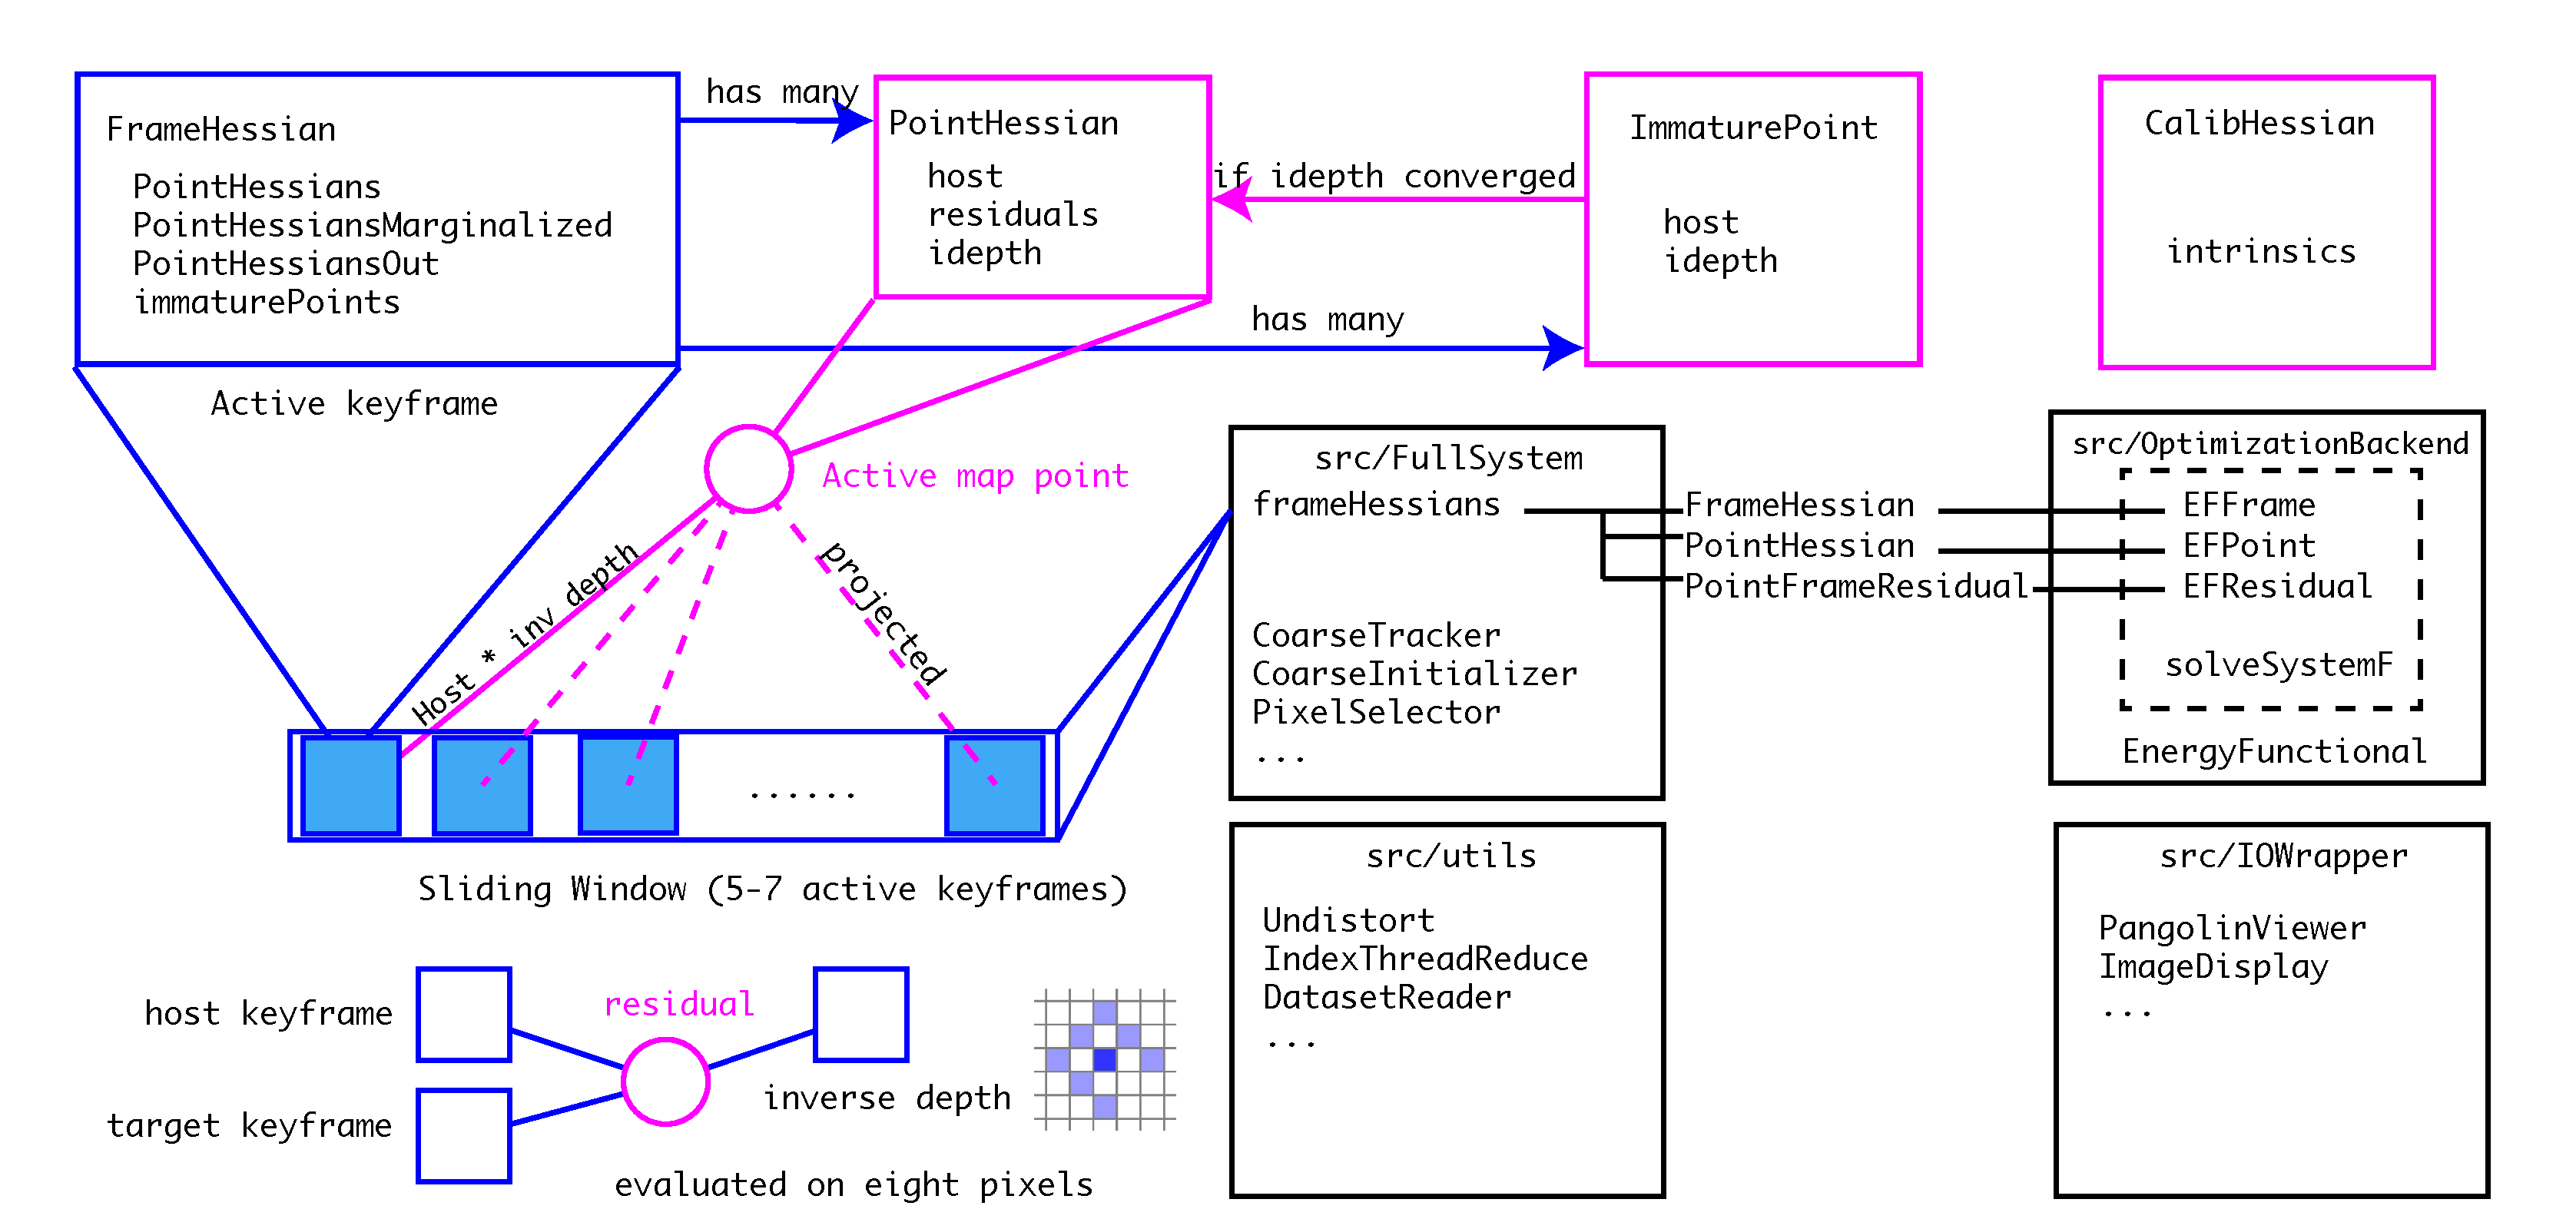
\includegraphics[width=1.0\textwidth]{figs/framework-dso-en}
	\caption{Framework of DSO.}
	\label{fig:framework-dso}
	\end{figure}
	First let's look at the general framework of DSO. I removed some unimportant classes and structures for the readers. See Fig.\ref{fig:framework-dso} for details (English version will be added later).
	
	The DSO code consists of four parts: the system and each algorithm are integrated in src/FullSystem, and the back-end optimization is located in src/OptimizationBackend, which constitutes most of the core content of DSO. Src/utils and src/IOWrapper are some undistorting, dataset reading and writing and visual UI code. Let's look at the core part of FullSystem and OptimizationBackend.
	
	As shown in the statements above, in FullSystem, DSO will maintain a sequence of keyframes inside a sliding window. The data of each frame is stored in the FrameHessian structure, and FrameHessian is a frame with state variables and Hessian information. Then, each frame also carries some map point information, including:
	\begin{enumerate}
	\item pointHessians is information about all active points. The so-called active points mean that they are in the field of view of the camera, and the residual term is still participating in the calculation of the optimization part;
	\item pointHessiansMarginalized is a map point that has been marginalized;
	\item pointHessiansOut is a map point that is marked to be an outlier;
	\item And immaturePoints is the information of immature map points.
	\end{enumerate}
	
	In monocular SLAM, all map points have only one 2D pixel coordinate at the beginning.  The depth is unknown. This point is called an immature map point in the DSO and stored in the ImmaturePoint class. As the camera moves, DSO tracks these immature map points on each image. This process is called \textbf{Trace} and is actually a process of searching along the epipolar line, very similar with svo's depth filter. The \textbf{Trace} process determines the inverse depth of each Immature Point and its range of variation. If the depth of the Immature Point (actually the inverse of the depth, ie the inverse depth) converges in the process, then we can determine the three-dimensional coordinates of this immature map point, forming a normal map point. A map point with three-dimensional coordinates, called PointHessian in DSO. In contrast to FrameHessian, PointHessian also records the three-dimensional coordinates of this point, as well as Hessian information.
	
	Unlike many other SLAM schemes, DSO uses a single parameter to describe a map point, its inverse depth. For most programs, such as ORB-SLAM, the coordinates of x, y, and z of the map point are recorded. The inverse depth parameterized form has the advantages of simple form, similar Gaussian distribution, and more robustness to distant scenes [5], but based on Bundle adjustment of inverse depth parameterization, each residual term needs to calculate one more than the usual BA. Jacobian matrix. In order to use the inverse depth, each PointHessian must have a host frame indicating that the point is back-projected from the frame.
	
	Thus, all information of the sliding window can be described by several FrameHessian, plus the PointHessian carried by each frame. All PointHessian can be projected in any frame from a host frame to create a residual term, which is recorded in PointHessian::residuals. Adding all the residuals constitutes an optimization problem that the DSO needs to solve. Of course, due to motion and occlusion, not every point can be successfully projected to all of the remaining frames, so we also need to set the state of each point as: valid /marginal/invalid. Points of different states are stored in the three containers of pointHessians/pointHessianMarginalized/PointHessiansOut of its host frame.
	
	In addition, DSO considers the camera's internal parameters, exposure parameters and other information as optimization variables. The camera internal parameters are expressed by the pinhole camera parameters fx, fy, cx, cy, and the exposure parameters are described by two parameters a, b. Please read the photometric calibration paper for details.
	
	The backend optimization part has separate Frame, Point, and Residual structures. Since the optimization goal of DSO is to minimize energy (similar to cost in Ceres), the classes related to the backend start with EF and correspond one-to-one with the instances stored in FullSystem, holding each other's pointers. The optimization part is managed by the EnergyFunctional class. It takes all the frames and points from FullSystem, optimizes them, and returns the optimization results. It also contains all the frame and point information in the entire sliding window and is responsible for handling the actual nonlinear optimization matrix operations.

	
	\subsection{Changes of LDSO}
	LDSO has made a lot of changes to the framework of DSO, in order to make the code structure more clear. The code structure of LDSO is mainly composed of the following folders:
	\begin{enumerate}
	\item include and src: header files and source code files.
	\item examples: some examples, such as running on Kitti or on EUROC.
	\item thirdparty: third-party libraries, sophus, dbow3 and g2o.
	\item vocab: a dictionary for loop detection
	\end{enumerate}
	The source code is divided into several subfolders:
	\begin{enumerate}
	\item In include/: the basic code structure, like Frame, Point, Feature, etc.
	\item include/frontend is the front-end related code, including the feature detection, tracking, as well as the system interface.
	\item Under include/internal is the backend and some internal algorithms, basically the content of the DSO, but for some reason I do not want to modify them.
	\item Under include/internal/OptimizationBackend is the backend that DSO implements itself. Since the general optimization libraries like Ceres or g2o do not natively support incremental optimization, DSO implements one by itself. This backend uses a lot of hacks \footnote{SSE acceleration of computing accumulated Jacobians, sharing some internal computation results, etc.}, making it hard to read and not general, but faster than the others.
	\end{enumerate}

	In the LDSO I extracted the main structure and made the whole logic look clearer. In general, in LDSO you will have some \textbf{Frame}s, and these \textbf{Frame}s will see some \textbf{Feature}s. If the depth of this \textbf{Feature} is correctly estimated, it will produce a corresponding \textbf{Point}. This structure is similar to SVO and is simple enough. So, if you want to get the entire track trajectory or save the entire map, just iterate through all the \textbf{Frame}s and \textbf{Point}s and save them.
	
	These classes are the simplest data structures of the program, of course, we still need to store some extra data in the actual operation. For example, for any \textbf{Frame}, I want to estimate its pose, then there may be an estimated state, a previously estimated state (for backup), and an increment. I put these in the internal/\textbf{FrameHessian}s, similar for \textbf{Point} to internal/\textbf{PointHessian}. In DSO, the old \textbf{Frame} and \textbf{Point} are immediately destructed from the inside, but in LDSO, I need to save them for rebuilding the map after loopback. So you can access the state of each \textbf{Frame} and \textbf{Point} at any time. \textbf{Frame} will hold a \textbf{FrameHessian} pointer and deconstruct it if not needed.
	
	LDSO also made some simplifications on the backend. In DSO, the backend is implemented by the EnergyFunctionals class. It uses some of its own EFPoints, EFFrame which have some overlap with the front end, so you often see a state data is passed from the front end to the backend, and passed back when calculation is finished. LDSO directly lets \textbf{EnergyFunctional} handle \textbf{FrameHessian} and \textbf{PointHessian}, and the results are stored directly in these classes, making the backend structure simpler.
	
	At the algorithm level, LDSO has a feature extraction and matching process, in the frontend/FeatureDetector, frontend/FeatureMatcher, to achieve the process of matching and extraction. Frontend/LoopClosing implements loopback detection. If the loopback is detected, then one of the Map classes completes the optimization of Sim3.
	
	LDSO saves the front/back position of the loopback for each frame. The optimized pose should be uniform in scale. Finally, the map corresponding to the optimized pose is displayed in the visualization window. I admit that the backend of DSO is difficult to change. I think the opinions of others in our group are the same.
	
	\subsection{Tracking}
	\begin{figure}[!thp]
	\centering
	\label{fig:frontend-dso}
	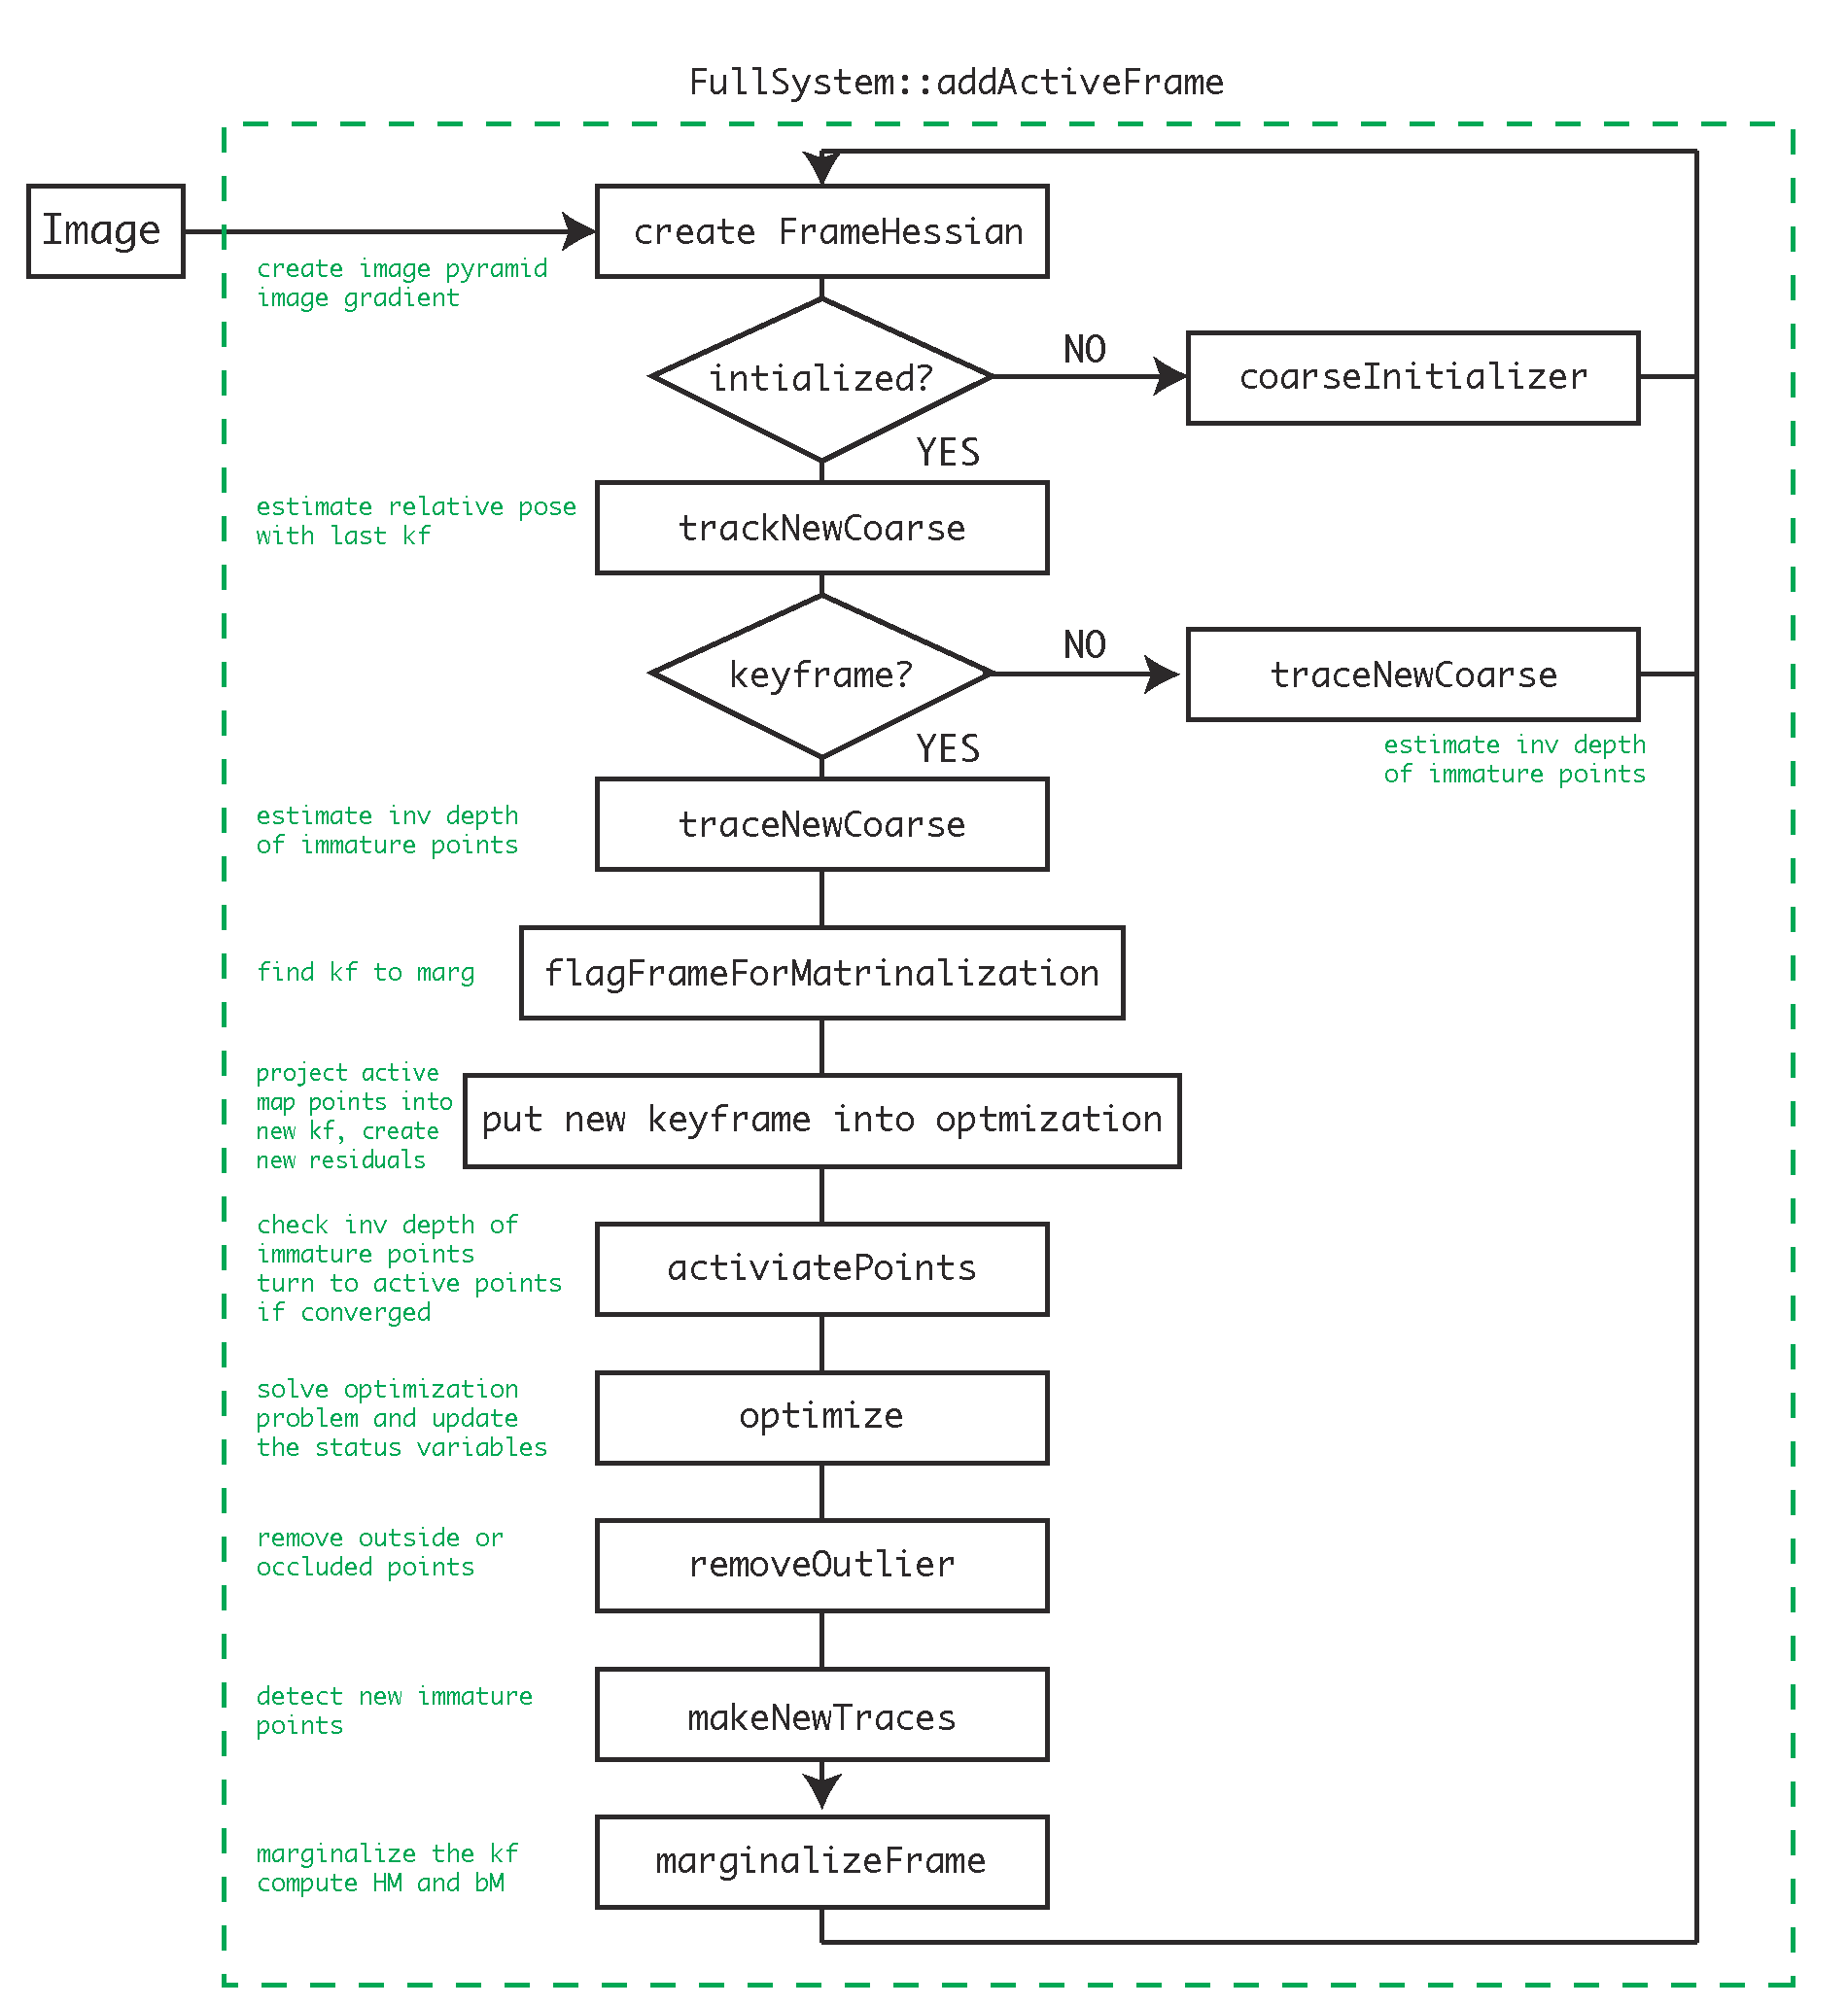
\includegraphics[width=0.8\textwidth]{figs/frontend-en}
	\caption{Pipeline of the frontend.}
	\end{figure}
	The frontend pipeline of DSO is illustrated in Fig.\ref{fig:frontend-dso}. Although the specific meaning of each step is not explained, the general flow of the DSO can be seen. From the above figure, we can briefly summarize the behavior of DSO:
	
	\begin{enumerate}
		\item For non-keyframes, the DSO only calculates its relative pose with the last keyframe, and updates the depth estimate for each immature point with the frame image;
		\item The backend only tackles the optimization of keyframes. In addition to some memory maintenance operations, the main processing for each key frame is: adding new residual items, removing the wrong residual items, and extracting new immature points.
		\item The entire process is in one thread, but there may be multi-threaded operations inside.
	\end{enumerate}
	
	\subsection{Backend}
	\subsubsection{Marginalization}
	The keyframes and the residuals of the map points, form the content of the entire sliding window. To optimize these frames and points, we will iterate using the Gauss-Newton or Levenberg-Marquardt methods. In each iteration, all residual terms can be combined into a large linear equation:
	\begin{equation}
	\mathbf{J}^T \mathbf{W} \mathbf{J} \delta \mathbf{x}=-\mathbf{J}^T \mathbf{W} \mathbf{r},
	\end{equation}
	Where $\mathbf{J}$, $\mathbf{W}$, $\mathbf{r}$ are the Jacobians, weights and residuals, respectively, and $\delta \mathbf{x}$ is the overall optimized update (innovation). The left side can be written as: $\mathbf{J}^T \mathbf{WJ}=\mathbf{H}$, which is the Hessian matrix. This matrix is maintained in memory throughout the optimization process. Note that this approach is different from some batch optimization systems like ORB-SLAM2. The back end of ORB-SLAM2 will continuously rebuild the entire optimization problem, solve it, and then fetch the optimized result, deconstruct the optimization problem. In DSO, since the problem is always maintained, subsequential optimizations can take advantage of previous results, or previous optimizations provide a prior for the next step. However, in order to maintain this information, DSO must manually add/delete each frame and point, unlike the ORB-SLAM2, which can directly start from any given frames and points.
	
	In batch bundle adjustment the $\mathbf{H}$ matrix has a very famous arrow-like shape as illustrated in Fig.\ref{fig:H-dso}. We can take advantage of this special sparse structure to accelerate the solving of the linear problem. This is somewhat misleadingly called as \textbf{Marginalization}, and implemented by sparse Schur complement (Schur trick) or sparse Cholesky decomposition. In the Schur trick, we marginalize all the points into the pose information, solve the pose equations, and then substitute the results into the points part, which can substantially reduce the computation time. 
	
	\begin{figure}[!thp]
		\centering
		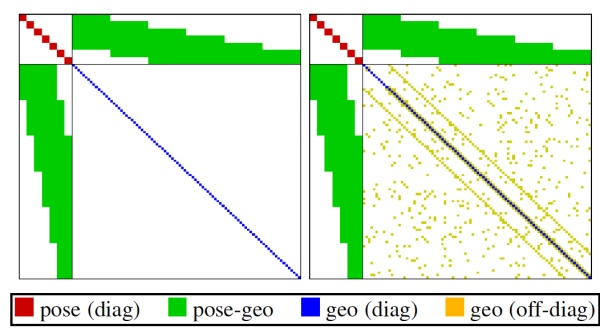
\includegraphics[width=0.8\textwidth]{figs/H.jpg}
		\caption{Arrow-like Hessian matrix in batch BA.}
		\label{fig:H-dso}
	\end{figure}
		
	DSO's BA, like the traditional BA, has the above steps. Therefore, when the DSO solves the BA in sliding window, it should marginalize all the points and calculates the optimized update amount in the pose part. However, unlike the traditional BA, the upper left part of the DSO is not a diagonal block matrix but added by a priori. In the traditional batch BA, this part is a diagonal block matrix. The main reason is that the prior motion of the camera movement is unknown, but in the sliding window of the DSO, this can be calculated by the previous motion information. The a priori here comes mainly from two parts:
	\begin{enumerate}
	\item When a point is marged, a priori is generated between the co-visible frames of the point;
	\item When a frame is marged, a priori is generated between other co-visible frames in the window;
	\end{enumerate}
	
	Here, "marginalization", the specific operation is the same as the marginalization mentioned above. That is to say, we use eliminate some part of the matrix via Shure complement. However, the actual meaning of the operation is different. In the marginalization of batch BA, we want to use marginalization to accelerate the solution of the linear problem, but after solving the problem, these frames and points still exist in the window! On the other side, the marginalization in the sliding window means that we no longer need this point/this frame. When it is marginalized, we pass its information to the motion priori, and will \textbf{no longer} use this point/this frame anymore! Readers must be clear about this difference, otherwise you will encounter problems when understanding DSO's code. We might call the former as "temporary marginalization" and the latter as "permanent marginalization" to distinguish them.
	
	So how does DSO permanently marginalize a frame or point? It follows the following guidelines:
	\begin{enumerate}
	\item If a point is no longer in the field of view of the camera, marginalize this point;
	\item If the number of frames in the sliding window has exceeded the set threshold, then select one of the frames for marginalization;
	\item When a frame is marginalized, the map points that use it as the host frame will be marged and will not participate in future calculations. Otherwise this point will form a priori with other points, destroying the sparse structure in BA. This strategy is similar with \cite{leutenegger2015keyframe}. Actually, many existing sliding window systems follows part of \cite{leutenegger2015keyframe}.
	\end{enumerate}
	
	The frame motion priori is stored in EnergyFunctional::HM and bM, and DSO directly adds this information into the BA linear equation. If you are using Ceres or other optimization libraries that don't support incremental solving, you probably need to pack this priori information into a fake residual block that is evaluated on all the active keyframes, like what okvis \cite{leutenegger2015keyframe} and VINS \cite{qin2017vins} does.
	
	\subsubsection{Null space and FEJ}
	In SLAM, in the GN or LM optimization process, the Hessian matrix may not be full ranked. The is called as null space, which means if you change the value of the state variable in this subspace, it will not affect the final cost of the objective function. In purely visual SLAM, the typical null space is the absolute scale of the scene and the absolute pose of the camera. In VIO, the null space also includes the yaw dimension. If you are using over-parametrized representations like quaternion as state variables, it will also lead to extra null spaces in Hessian matrix. It is conceivable that if the camera and the map are simultaneously enlarged by one scale, or rotated and translated at the same time, the entire objective function should not change. The null space also exist in the marginalized motion priori. For example, if the marginalized keyframe has no co-visible features with another active keyframe, then the Jacobian matrix will be zero block between them and make a zero block in the Hessian. In okvis \cite{leutenegger2015keyframe} the author made a eigen value decomposition of the marginalization Hessian and eliminate those subspaces that have very small eigen values.  The existence of null space also leads to the solution of the linear equation is not unique during the optimization process. Although the step size of each iteration is small, but as time going, it is easy for the whole system to wander in these zero spaces, causing the estimation to drift.
	
	On the other hand, due to the existence of marginalization, if a point is marginalized, its Jacobian matrix should be fixed at the moment of marginalization, while the Jacobian of other points will be updated over time. The timing at which different variables are linearized throughout the system is different. This leads to the dimensionality reduction of the null space - the zero space that should exist, but disappears due to the different linearization moments! And our estimates will become too optimistic. %DSO's author has shown a very intuitive example about this phenomenon, see Fig.\ref{fig:nullspace-dso}. 
% TODO: clarify use with Jakob and add back

%	\begin{figure}[!thp]
%		\centering
%		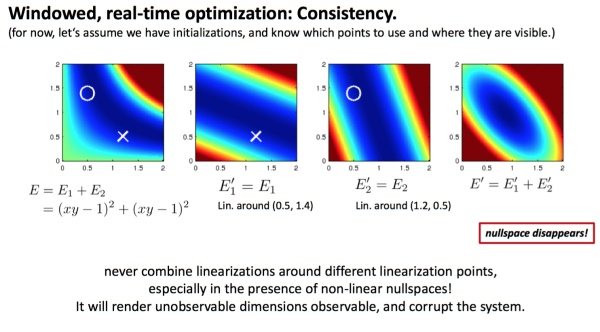
\includegraphics[width=0.8\textwidth]{figs/nullspace.jpg}
%		\caption{Null space disappears if linearization point is different.}
%				\label{fig:nullspace-dso}
%	\end{figure}

	In this example, we minimize an energy function of $E=E_1+E_2=(xy-1)^2+(xy-1)^2$. Obviously, the curve xy=1 is the optimal solution, which is exactly one-dimensional null space. However, if $E_1$ and $E_2$ are linearized at different points, the obtained E may cause the zero space of this dimension to disappear (as shown in the figure), when the optimal solution becomes a point.
	
	Therefore, in DSO the Jacobi of geometry and luminosity is calculated only at the initial moment of optimization, and they remain unchanged during the following iterations, namely First-Estimate-Jacobian. FEJ forces each point to be linearized at the same time, thus avoiding the problem of null space dimensionality reduction and reducing the amount of computation. For each map point in the DSO, eight residuals are generated from the previously defined pattern, and these residuals also share the FEJ. Since the geometric and photometric functions are relatively smooth, the FEJ approximation is very useful in practice. Actually the direct tracking part of SVO \cite{forster2014svo} also makes use of FEJ, where the Hessian matrix is pre-calculated and only the residuals are updated during the iterations. 
			
	\bibliographystyle{plain}
	\bibliography{reference}
	
\end{document}
